\documentclass[11pt,a4paper]{article}
\pdfminorversion=7

\usepackage[margin=2.5cm]{geometry}
\usepackage[T1]{fontenc}
\usepackage[utf8]{inputenc}
\usepackage{lmodern}
\usepackage{setspace}
\usepackage[mathlines]{lineno}
\usepackage{graphicx}
\usepackage{booktabs}
\usepackage{longtable}
\usepackage{array}
\usepackage{multirow}
\usepackage{amsmath}
\usepackage{amssymb}
\usepackage{siunitx}
\usepackage{float}
\usepackage{placeins}
\usepackage{adjustbox}
\usepackage{hyperref}
\usepackage[round,authoryear]{natbib}
\usepackage{caption}

\hypersetup{colorlinks=true,linkcolor=black,citecolor=black,urlcolor=blue}

\newcommand{\StdTableInput}[1]{%
  \begingroup
  \singlespacing
  \footnotesize
  \setlength{\tabcolsep}{4pt}%
  \renewcommand{\arraystretch}{1.1}%
  \begin{adjustbox}{max width=\linewidth}
    \input{#1}%
  \end{adjustbox}
  \endgroup
}

\title{Anatomical prediction of sacroiliac motion and its load-dependent limits}
\author{%
Petr Heny\v{s}$^{1,*}$, Niels Hammer$^{2}$\\
\small $^{1}$Institute of New Technologies and Applied Informatics,\\
\small Faculty of Mechatronics, Informatics and Interdisciplinary Studies,\\
\small Technical University of Liberec, Studentsk\'a 1402/2, 461~17 Liberec, Czech Republic\\
\small $^{2}$Division of Macroscopic and Clinical Anatomy,\\
\small Gottfried Schatz Research Center, Medical University of Graz,\\
\small Auenbruggerplatz~25, 8036~Graz, Austria\\
\small $^{*}$Corresponding author: Petr Heny\v{s} (\texttt{petr.henys@tul.cz})%
}
\date{}

\renewcommand{\topfraction}{0.95}
\renewcommand{\bottomfraction}{0.85}
\renewcommand{\textfraction}{0.05}
\renewcommand{\floatpagefraction}{0.85}
% Keep float-only pages compact instead of vertically spreading figures.
\makeatletter
\setlength{\@fptop}{0pt}
\setlength{\@fpsep}{18pt}
\setlength{\@fpbot}{0pt plus 1fil}
\makeatother

\begin{document}
\doublespacing
\begingroup
\singlespacing
\maketitle
\endgroup
\linenumbers

\begin{abstract}
Pelvic mechanical response reflects anatomical variation expressed through a specified load path. We examined sacroiliac joint responses in 278 imaging-derived pelves under five standardized loading configurations and in matched geometry--bone-density variants. Redistributing the same 800~N total acetabular force from bilateral to unilateral support amplified motion and asymmetry; transverse force pairs applied at different sites produced distinct component patterns. Adjustment for pelvic volume and a selected morphometric triad substantially attenuated age-adjusted sex-associated translation differences under localized loading, with all fully adjusted confidence intervals spanning zero. Preserving individual geometry while standardizing the bone-density field retained subject-specific translation closely (RMSE $\leq0.028$~mm; minimum identity-line $R^2=0.946$). In retrospective adjusted log--log analyses, all 20 sex-specific volume--motion slopes were negative after multiplicity correction. Bilateral standing-like slopes were numerically near simple fixed-force dimensional reference values, whereas several localized-load estimates were numerically steeper. These conditional relations describe size-dependent response under identical prescribed forces across subjects within each load case. Together, the comparisons support a description of pelvic mechanics organized by anatomical scale and individual architecture, with load path determining their mechanical expression. Sex-associated contrasts varied with anatomical adjustment and loading configuration. Interpretation remains conditional on passive static mechanics, the implemented density--modulus law and fixed cartilage, ligament and pretension parameters.

\end{abstract}

\noindent\textbf{Keywords:} functional morphology; cross-validation; force redistribution; directional cancellation; finite-element analysis

\section{Introduction}
The sacroiliac joints (SIJs) transfer load between the spine and lower limbs through a ring stabilized by articular geometry, ligaments and muscular compression \citep{Snijders1993,Vleeming2012,Hammer2013}. Small three-dimensional joint movements vary substantially between individuals \citep{Hammer2019}. Understanding this variation requires more than describing average mobility: an anatomical account should specify how much of the response can be predicted from a small set of measurements and which information is lost when the full pelvic geometry is reduced to those measurements.

Pelvic variation includes overall size, inlet and midpelvic proportions, pubic arch geometry and local SIJ morphology. Sex-associated dimensions follow distinct developmental trajectories \citep{Huseynov2016}, and pelvic shape covaries with stature \citep{Fischer2015}. Overall height-to-width proportions have a substantial allometric component, whereas subpubic-angle dimorphism is predominantly non-allometric \citep{Fischer2017}; local iliac auricular shape also differs between sexes \citep{Nishi2020}. These observations motivate anatomical predictors that represent scale and complementary dimensions of the ring. They do not establish that a few dimensions reproduce the mechanical information carried by a complete geometry.

Comparative finite-element analysis can connect anatomical variation to mechanical function, provided that the loading question and the distinction between size and shape are explicit \citep{Dumont2009}. A previous population study of 281 CT-derived pelvic models related auricular surface morphology and cartilage dimensions to SIJ stress and deformation \citep{HenysHammer2025}. The present 278-subject cohort is a subset of that CT collection, rather than an independent anatomical sample. Here the question concerns relative joint kinematics under five loading configurations, prediction in held-out subjects, and a controlled test of the information needed when load application is redistributed. The source anatomy overlaps; the predictive assessment and load-mixture experiment address questions beyond the earlier morphology--stress analysis.

Sex-associated SIJ mobility has been reported in representative male/female models \citep{Joukar2018}, upright MRI \citep{Tani2023}, and cadaveric measurements \citep{Shin2024}. In the present passive model, however, sex is a statistical group label: geometry and density are individualized, while cartilage, ligament and pretension parameters are shared. Simulated group differences therefore arise through those represented inputs. The useful question is whether explicit anatomical measurements capture their predictive information, and whether adding the sex label improves prediction after anatomy is included. Attenuation of an adjusted group coefficient alone cannot establish this predictive sufficiency or biological sex equivalence.

Loading provides a second limit to anatomical reduction. For fixed linearized stiffness, displacement fields superpose, but their magnitudes do not generally do so. Forces applied at different parts of the ring can produce joint-displacement vectors that reinforce or oppose one another. A model describing only response magnitude under each loading configuration may therefore lose information required to combine loads, even when the geometry is unchanged. This distinction supplies a testable mechanism for a failure of scalar response reduction. It is separate from the cross-subject errors of an anatomical predictor.

Material representation also sets the scope of prediction. Ligament pretension affects SIJ response \citep{Heyland2025}, and reductions in bone stiffness can alter modeled motion \citep{Fan2026}. Matched variants retaining either individual geometry or individual bone density allow assessment of a geometry-preserving density simplification, with soft-tissue parameters held fixed. Such comparisons quantify approximation error for specified endpoints; they do not establish a universal hierarchy of anatomical and material effects.

We asked how far pelvic size and three anatomical measures predict population SIJ motion across loading configurations, and what directional mechanism limits transfer to a redistributed load. Using 278 geometries from the BoneDat workflow \citep{HenyssKuchar2025BoneDat}, we compared size-based and triad-augmented predictions in repeated subject-held-out cross-validation. The triad comprises inlet AP depth, interspinous width and subpubic angle. Additional sex terms and all eight available measures were assessed as benchmarks. We then redistributed fixed transverse forces between the internal ring and ischial tuberosities and compared scalar and signed-vector combinations against kinematics re-extracted from the mixed FE fields. All analyses were retrospective. Predictions concern the represented passive mechanics and loading configurations; the force pairs are mechanical probes, and do not represent fetal passage or maternal soft-tissue deformation during childbirth \citep{ChenGrimm2021}.

\section{Materials and methods}
\subsection{Cohort and provenance}
The cohort comprised 278 pelvic models (150 female, 128 male), aged 16--91 years (mean $\pm$ SD: $53.9\pm19.3$ years), using the BoneDat morphology workflow \citep{HenyssKuchar2025BoneDat}. These subjects are a subset of the 281-subject CT collection used in the earlier auricular morphology study \citep{HenysHammer2025}; they are not an independent replication cohort. The present analysis uses the 278 subjects represented in the matched geometry--density simulation archives. Demographic, morphometric and size tables were joined by subject identifier. Eight morphometric variables and the kinematic outcomes were complete for the included cohort (Table~\ref{tab:cohort}). Ethical approval was granted by University Hospital Hradec Kr\'alov\'e, reference 202411IO3P, with waiver of informed consent.
\begin{table}[htbp]
\centering
\caption{Demographic and morphometric characteristics. Values are mean $\pm$ SD; linear dimensions and the subpubic angle are measured from mapped landmarks. Bony pelvic volume sums the selected left and right hip-bone bodies and sacrum.}
\label{tab:cohort}
\StdTableInput{tables/generated/table1_cohort.tex}
\end{table}

\subsection{Anatomical dimensions and their landmarks}
Figure~\ref{fig:morphometry} shows all eight morphometric measures in Table~\ref{tab:cohort}, using the template landmarks from the measurement workflow. Each of the seven linear dimensions is the three-dimensional Euclidean distance $d=\|\mathbf p_2-\mathbf p_1\|$, rather than its projection into a display plane. The subpubic angle uses the second of three landmarks as its vertex:
\begin{equation}
\alpha_{sub}=\arccos\!\left[\frac{(\mathbf p_1-\mathbf p_2)\cdot(\mathbf p_3-\mathbf p_2)}{\|\mathbf p_1-\mathbf p_2\|\,\|\mathbf p_3-\mathbf p_2\|}\right],
\end{equation}
with numerical clipping to $[-1,1]$ and conversion to degrees. The landmark labels are local to each measurement. Landmarks were mapped from the template to each subject; interpolation settings and numerical checks are given in Appendix~\ref{app:implementation_checks}. Total mapped bony pelvic volume is the summed geometric volume of the selected left and right hip-bone bodies (LI and RI in the implementation) and sacrum, expressed in cm$^3$. It excludes the lumbar vertebrae and pelvic canal space and is not a direct measure of cortical-tissue volume. Supplementary Figure S2 illustrates these three bone bodies, the rotational coordinates and point-translation definition.

\begin{figure}[p]
\centering
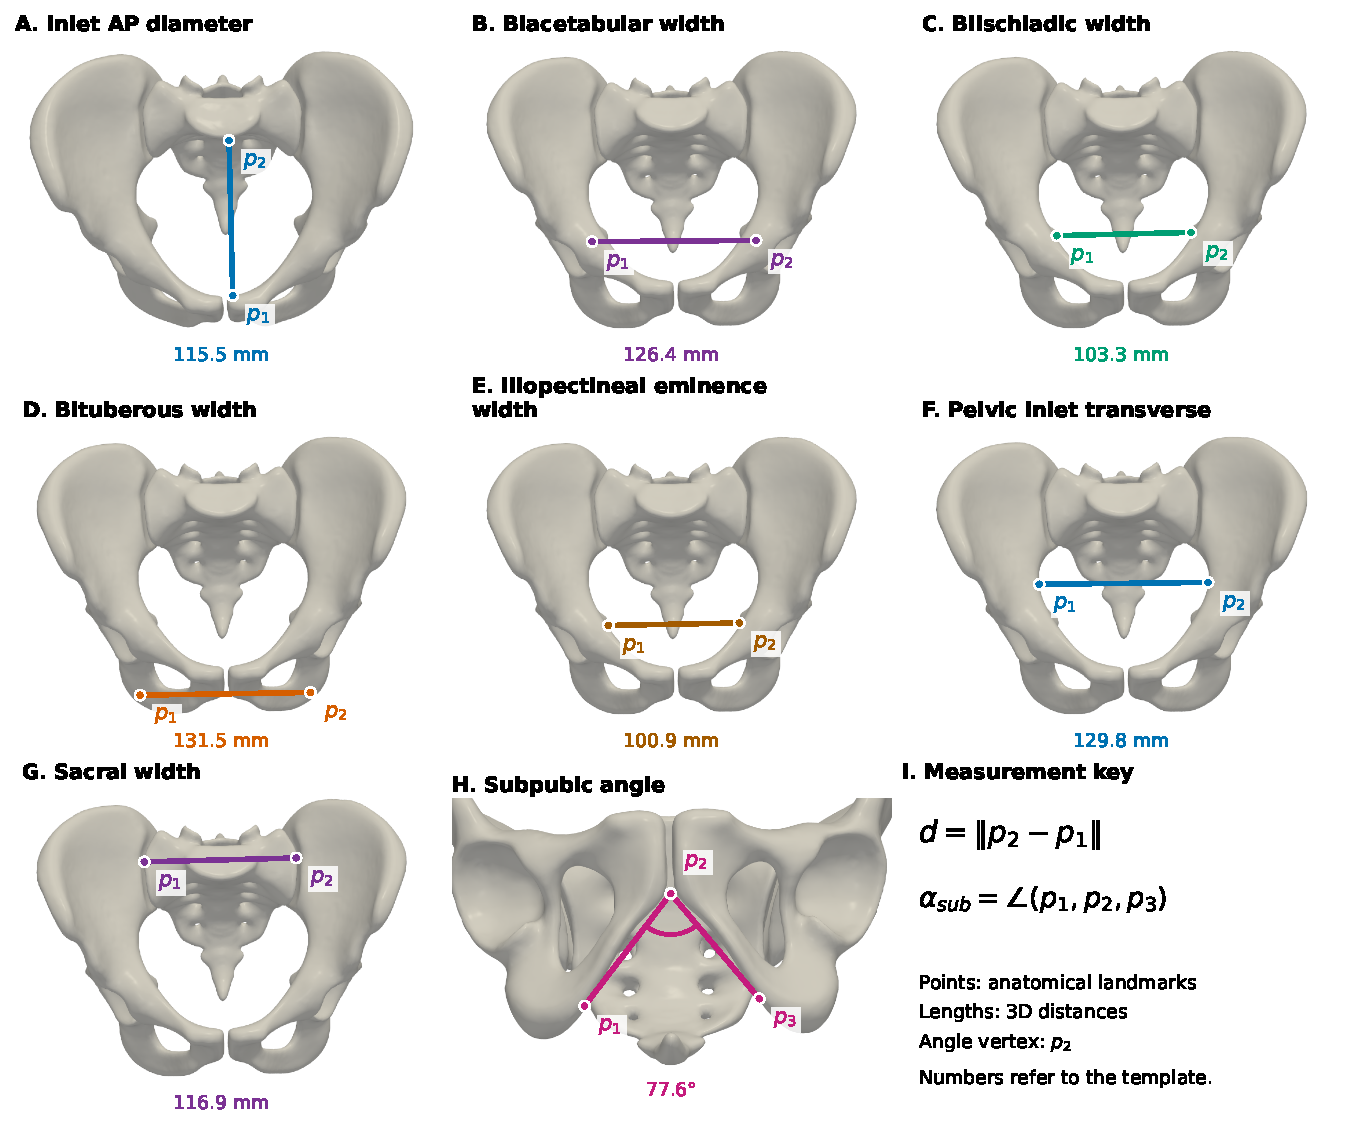
\includegraphics[width=\textwidth,height=0.76\textheight,keepaspectratio]{figures/Fig_morphometric_landmarks.pdf}
\caption{\textbf{Anatomical landmarks for all morphometric measures.} (A--G) Landmark pairs define the seven linear dimensions in Table~\ref{tab:cohort}. (H) The subpubic angle has vertex $p_2$ and arms toward $p_1$ and $p_3$; the view is normal to their plane. (I) Measurement definitions and landmark key. Markers and segments are overlaid on the reference pelvic geometry to keep internal landmarks visible. Values describe the template, not cohort averages. Lengths are measured in three dimensions; each camera direction is perpendicular to its measurement segment. Panels use different views and magnifications.}
\label{fig:morphometry}
\end{figure}

\subsection{Finite-element model}
The simulations used DOLFINx 0.10 on a mesh with 166,808 cells and 48,291 nodes. Small-strain linear elasticity was discretized with four-node tetrahedra and continuous, first-order Lagrange displacement and geometry fields; material properties were cellwise constant (DG0). PETSc used a direct MUMPS LU factorization on the shared reference domain (Appendix~\ref{app:implementation_checks}). Subject anatomy was established by bijective anatomical registration and represented on the FE discretization by $\mathbf{x}=\mathbf{X}+\boldsymbol{\phi}_i(\mathbf{X})$, using radial basis function (RBF) interpolation of the established registration displacement map. Spatial gradients and integration measures were pulled back to the reference domain \citep{BonetWood2008}. This interpolation approximates individual anatomy on a shared discretization and does not reproduce cortical boundaries exactly.

Experimental relationships between bone density and stiffness motivate density-dependent material assignment \citep{Keller1994}. Bone stiffness was assigned using the following bone-modulus approximation:
\begin{equation}
E/\mathrm{MPa}=\begin{cases}
2398, & \rho_{\mathrm{ash}}\le0.486,\\
10200\rho_{\mathrm{ash}}^2, & \rho_{\mathrm{ash}}>0.486,
\end{cases}
\qquad \rho_{\mathrm{ash}}=(\rho+0.09)/1.14,
\end{equation}
where numerical density values are in g\,cm$^{-3}$ and $\rho$ denotes the mapped hydroxyapatite-density input. The implemented approximation comprises this equation, density conversion and low-density floor. The constant low-density branch suppresses modulus variation below its threshold. Bone Poisson ratio was 0.30. Both SIJ cartilage and pubic symphysis used $E=1.0$~MPa and $\nu=0.45$ in all three model variants. These nominal choices were not calibrated to individual subjects.

Ligaments were assembled as linear spring stiffness matrices with a geometric stiffness contribution from prescribed pretension and a pretension force vector. The implementation does not update a tension-only active set during the static solve. Bilateral anterior SIJ, posterior SIJ, interosseous, sacrospinous and sacrotuberous bundles and the pubic bundle were included. Per-bundle stiffnesses were respectively 1400, 5600, 200, 3000, 3000 and 1000~N/mm; total pretension was 20~N per bundle. Each bundle's parameters were divided among its segments. Bone--cartilage interfaces were conforming; frictional contact and muscle activation were not modeled.

\subsection{Loads and constraints}
The superior S1 endplate was constrained using a surface penalty $\gamma=10^6$~N/mm$^3$ (Appendix~\ref{app:mathematical_formulation}). Figure~\ref{fig:overview} shows the load application sites; Table~\ref{tab:loads} gives force vectors in the simulation's global coordinates; these must be distinguished from the subsequently constructed pelvis-aligned reporting frame. SP2leg applies $+400$~N vertically to each acetabulum, and SP1leg applies $+800$~N to the right acetabulum. LAB1 applies opposing ML forces of $\pm400$~N to the internal ring surfaces; LAB2 applies the same signed pair to the ischial tuberosities; LAB3 applies opposing AP forces of $\pm400$~N at the pubis and sacrococcygeal junction. The reference template places both left application patches at greater global $x$ than their right counterparts; thus both ML pairs point outward in that template, consistent with outward loading at both sites. We name the cases by application site because a force direction does not establish the direction of joint motion.

Surface tractions were normalized by mapped surface area, giving identical prescribed force resultants across subjects. LAB force pairs have zero net force, whereas standing cases have an 800~N net vertical force balanced by the sacral constraint. Equal sums of force magnitudes do not imply equal moments, work, or physiological demand. The analyses compare responses to these standardized mechanical probes. All load cases include the prescribed ligament pretension.
\begin{table}[htbp]
\centering
\caption{Standardized loads in global simulation coordinates. LAB1--LAB3 are independent mechanical proxies.}
\label{tab:loads}
\StdTableInput{tables/generated/table2_loads.tex}
\end{table}

\subsection{Reference configuration and SIJ kinematics}
The kinematic analysis compares each unloaded mapped surface $\mathbf{x}^0_i=\mathbf{X}+\boldsymbol{\phi}_i$ with its loaded surface $\mathbf{x}^1_{i\ell}=\mathbf{x}^0_i+\mathbf{u}_{i\ell}$. The reference is the anatomical configuration with zero elastic displacement; a separately equilibrated pretension-only configuration is not used. Absolute motion therefore describes the combined external-load and prescribed-ligament-pretension solution relative to this anatomical reference. Pretension is a model assumption, not an experimentally measured subject-specific value. Correspondence and pairing checks are documented in Appendix~\ref{app:implementation_checks}.



Relative ilium-to-sacrum motion was estimated using trimmed Kabsch registration of opposing surface regions within 5~mm, with a minimum of 80 nodes per region. The underlying least-squares rigid fit follows \citet{Kabsch1976}; trimming and ROI selection are implementation choices. Before registration, the inverse least-squares affine sacral map was applied to all loaded points. This removes sacral affine strain as well as rigid drift; the resulting quantities are affine-corrected relative motion, rather than unmodified physical joint displacement. The available rigid-only sensitivity check is reported below.

Motion was expressed in a pelvis-aligned ML/AP/CC frame, not a local articular normal/tangent frame. Fixed-axis Cardan $xyz$ angles satisfy $R=R_zR_yR_x$. The bilateral mean of the Euclidean norms of these angle triplets is denoted $|\boldsymbol{\theta}|$; this is a small-angle summary, not the exact invariant rotation angle. Translation $|\mathbf d|$ is the bilateral mean of the norms of relative displacements evaluated at the sacral ROI centroid. Component summaries are bilateral means of absolute values. In particular, $|\theta_x|$ does not distinguish nutation from counternutation, and $|d_{ML}|$ is not a measurement of joint gapping. Translation-magnitude asymmetry is $\big|\|\mathbf d_L\|-\|\mathbf d_R\|\big|$.

\subsection{Matched variants and variance ratios}
The full variant uses subject-specific geometry and bone density. The geometry-preserved / standardized-density variant (G) retains subject geometry, including scale, and uses the spatially varying pointwise population-median density field; it is not homogeneous bone. The density-preserved / template-geometry variant (D) uses subject density on the template geometry. Cartilage and ligament parameters remain nominal in all variants.

For each load and endpoint we calculated $100V_G/V_{full}$ and $100V_D/V_{full}$, with 2000 paired subject bootstrap samples \citep{EfronTibshirani1994}. These non-additive ratios can exceed 100\% and neither estimate causal variance fractions nor separate geometry--material interactions. Geometry-preserved/full agreement was also assessed by RMSE, MAE and identity-line $R^2=1-\sum_i(Y_{G,i}-Y_{full,i})^2/\sum_i(Y_{full,i}-\bar Y_{full})^2$.

\subsection{Prediction from size and a limited anatomical description}
The central predictive comparison used load-specific OLS models for $\log Y$, with $Y$ equal to rotation or translation magnitude. The size model used age and $\log V$. The triad model added inlet AP diameter, interspinous width and subpubic angle. Two benchmark models added, respectively, female sex and its interaction with $\log V$ to the triad, or replaced the triad with all eight available morphometric measures. Sex was not an independent parameter of the FE constitutive model. Predictor sets were fixed for this retrospective comparison; the original selection of the triad was not repeated within validation folds.

We used ten repeats of ten-fold cross-validation, stratified by sex at the subject level (random seed 20261002 plus repeat index). The same folds were used for every outcome, load and predictor set. All observations of a held-out subject were excluded from training; load-specific models were fitted only to the training subjects. Predictors were standardized using each training fold. Predictions on the arithmetic outcome scale used a training-only smearing factor, $\widehat Y=\exp(\widehat{\log Y})\,n_{train}^{-1}\sum_{i\in train}\exp(e_i)$. Each fold fitted the predefined predictor set without further feature selection or hyperparameter tuning.

Reported RMSE and MAE pool all held-out predictions across repeats. Prediction $R^2=1-\operatorname{mean}_{i,r}(Y_i-\widehat Y_{ir})^2/\operatorname{var}_i(Y_i)$ uses the cohort outcome variance, separately for each load and endpoint; it is not training fit. Paired gains compare models on identical held-out observations. Pointwise 95\% bootstrap intervals use 3000 subject resamples of repeat-averaged squared errors, preserving pairing across predictor sets. They condition on fitted cross-validation predictions and do not include the uncertainty of refitting or retrospectively selecting the triad. Repeated folds are not treated as independent samples. Validation addresses new subjects from the represented population under each specified load, not external specimens or unseen loading configurations.

\subsection{Controlled test of a directional limit to scalar prediction}
We redistributed each 400~N transverse side force between the internal-ring (LAB1) and ischial (LAB2) patches. At fraction $w\in\{0,0.25,0.5,0.75,1\}$, LAB1 patches receive fraction $1-w$ and LAB2 patches fraction $w$. Each side's total force and direction remain unchanged; geometry, density, constraints and linearized tissue stiffness remain fixed. Because both endpoint solutions contain the same pretension and the weights sum to one, the displacement field
\begin{equation}
\mathbf u_i(w)=(1-w)\mathbf u_{i,LAB1}+w\mathbf u_{i,LAB2}
\label{eq:mixture_field}
\end{equation}
solves the corresponding mixed-force problem in the implemented linear system. The experiment uses exact field superposition and requires no new FE factorization.

For all 278 subjects, motion was re-extracted from the mixed fields using the original affine-corrected, trimmed-Kabsch definitions and each subject's fixed unloaded ROI. Both endpoint weights reproduced the archived corrected rotations and translations to absolute and relative tolerances of $10^{-8}$. A scalar endpoint estimate combines bilateral translation magnitudes, $S_i(w)=(1-w)Y_{i,LAB1}+wY_{i,LAB2}$. A signed-vector endpoint estimate first combines each side's reported displacement vectors and then takes their bilateral mean norm, $D_i(w)=\frac12\sum_{s=L,R}\|(1-w)\mathbf d_{i,LAB1,s}+w\mathbf d_{i,LAB2,s}\|$.

The vector norm contains the cross-term $2w(1-w)\mathbf d_{LAB1,s}\cdot\mathbf d_{LAB2,s}$, which scalar magnitudes cannot identify. We quantified the reduction relative to scalar combination as $100[1-Y_i(w)/S_i(w)]$ and compared scalar and vector RMSE against re-extracted $Y_i(w)$. Signed-vector combination is an approximation at the level of these fitted kinematic outputs, despite exact superposition of the underlying FE fields; its error was measured rather than assumed zero. Both endpoint estimates use individual FE endpoint information and are mechanism diagnostics, not anatomy-only held-out predictions. This experiment tests transfer to a controlled load mixture; it does not identify the causes of residual cross-subject prediction error. Bootstrap intervals for median reduction use 3000 subject resamples.

\subsection{Statistical analysis}
All comparisons were retrospective and were not preregistered. Held-out prediction gains and the controlled load-mixture experiment form the central analyses; anatomical-adjustment, load-profile and density-variant comparisons provide context and delimit their interpretation. Distributions are summarized by medians and interquartile ranges. Paired component contrasts use $\Delta_{i\ell,k}=|d_k|_{i\ell}-|d_k|_{i,SP2leg}$, with 3000 subject bootstrap samples for median confidence intervals and two-sided exact binomial sign tests (zero differences excluded). Wilcoxon signed-rank statistics \citep{Wilcoxon1945} are retained in the machine-readable output as a sensitivity diagnostic, but are not used for primary inference because asymmetric differences can yield a signed-rank result that disagrees with the direction of the median. Benjamini--Hochberg correction was applied to the 12 component comparisons \citep{BenjaminiHochberg1995}. Bilateral versus unilateral support uses a separate three-test family for rotation magnitude, translation magnitude and translation asymmetry. Direct LAB2-minus-LAB1 contrasts use a separate three-component family. Prediction-gain intervals are descriptive, pointwise comparisons of paired held-out errors; no multiplicity-adjusted hypothesis tests were applied to them.

For each LAB case, nested OLS models used HC3 covariance \citep{MacKinnonWhite1985}:
\begin{align}
\mathrm{M0}:\quad Y&=\beta_0+\beta_s\mathrm{Female}+\beta_a\mathrm{Age}_z+\epsilon,\label{eq:m0}\\
\mathrm{M1}:\quad Y&=\mathrm{M0}+\beta_v\log(V)_z,\label{eq:m1}\\
\mathrm{M2}:\quad Y&=\mathrm{M1}+\beta_{AP}\mathrm{AP}_z+\beta_b\mathrm{Biischiadic}_z+\beta_p\mathrm{Subpubic}_z.\label{eq:m2}
\end{align}
Here model addition denotes addition to the linear predictor. Female is coded 1 and male 0; continuous predictors are standardized using cohort sample SDs. M2 contains no sex--volume interaction. FDR correction covers its six sex coefficients (two outcomes by three loads). M0/M1 and coefficient attenuation are descriptive. VIFs quantify collinearity without treating a threshold as proof of identifiability. The triad describes inlet depth, interspinous midpelvic width and the anterior pubic arch; it was selected for this retrospective analysis. Pooled and sex-stratified Spearman correlations are exploratory, not evidence of mediation.

Pooled OLS models include load, sex, age, log volume, the morphometric triad, load--volume interactions and a sex--volume interaction, with covariance clustered by the 278 subjects \citep{CameronMiller2015}. A main volume coefficient therefore refers to male SP2leg, not an overall pooled slope. FDR is applied within each outcome's pooled coefficients. Robust Wald statistics are not converted to partial variance-explained measures.

Exploratory load-specific association models regress $\log Y$ on $\log V$, sex, their interaction, age and the triad. Male and female slopes are $\beta_v$ and $\beta_v+\beta_{v:s}$; HC3 covariance supplies 95\% Wald intervals. FDR covers 20 sex-specific slope tests, with a separate family of ten interaction tests. Failure to reject an interaction is not evidence of equal slopes. A matched specification omitting the triad assesses the dependence of volume coefficients on anatomical adjustment (Supporting Information, Table S13). Neither specification represents uniform geometric scaling. The alternative $\log(\mathrm{scale})$ model is an algebraic reparameterization because $\log V=3\log(\mathrm{scale})+\log V_{template}$; it is not an independent robustness test. A sensitivity analysis added a quadratic age term to the nested sex models and the conditional volume models (Supporting Information, Tables S7--S8). Sample confidence intervals do not include uncertainty in loads, constitutive choices, segmentation or boundary conditions.

\subsection{AI assistance and reproducible postprocessing}
OpenAI Codex (GPT-6, OpenAI; used in October 2026) assisted with development of Python code for held-out prediction, load-mixture postprocessing, statistical checks and visualization. The calculations used the archived subject data and displacement fields described above; the language model itself was not a fitted predictor of SIJ motion. Predictions were computed by OLS and motion under force redistribution was re-extracted from the mixed FE fields, using the stated folds, seeds, interpolation and kinematic definitions. New result figures were rendered from these numerical outputs with Matplotlib, rather than generated as synthetic images. Independent raw-predictor statsmodels refits reproduced all 4000 held-out regressions, and both force-mixture endpoints reproduced the archived components for all 278 subjects at the stated tolerances. The authors reviewed the code-assisted results and approved their interpretation and the final manuscript.

\FloatBarrier
\section{Results}

\begin{figure}[htbp]
\centering
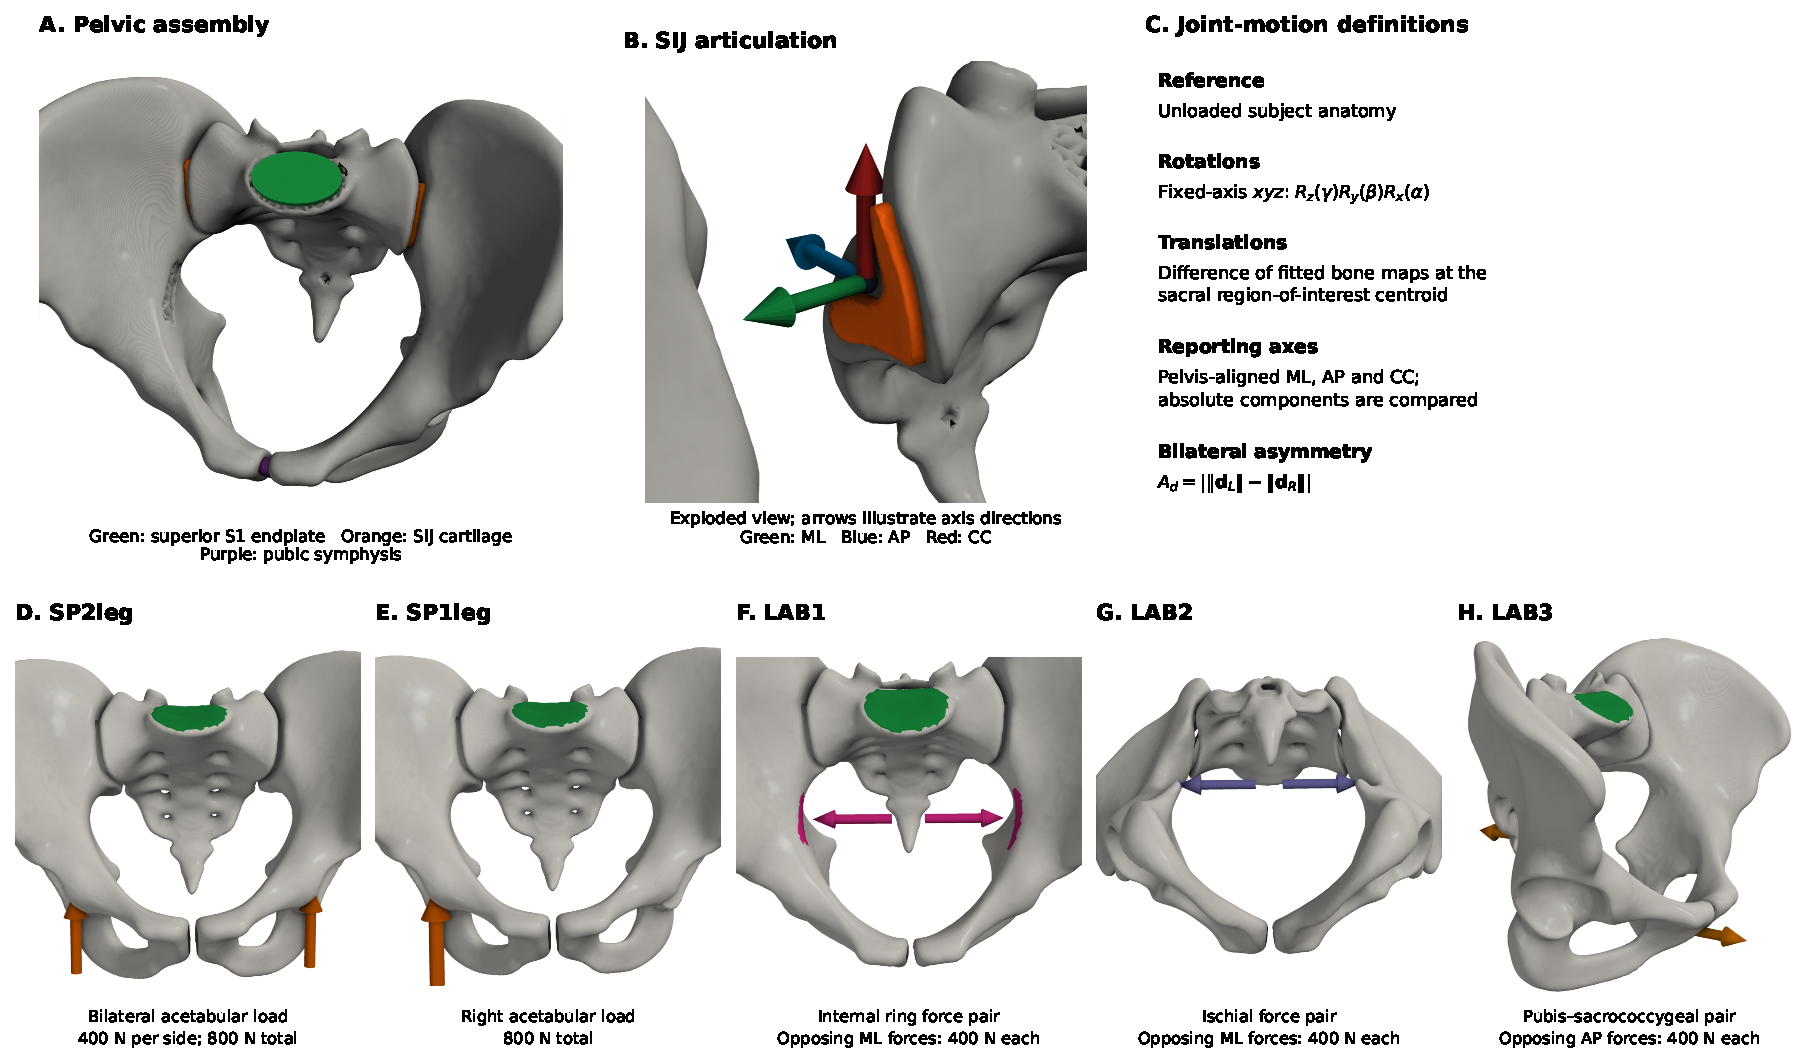
\includegraphics[width=\textwidth,height=0.67\textheight,keepaspectratio]{figures/Fig1_anatomy_coordinates_loads.pdf}
\caption{\textbf{Anatomy, motion definitions and load application.} (A) Pelvic assembly: green denotes the superior S1 endplate constraint, orange SIJ cartilage and purple the symphysis. (B) Exploded articulation with illustrative axis directions; these arrows do not define the subject-specific PCA frame or anatomical signs. (C) Rotational and translational reporting conventions. (D,E) Bilateral and unilateral acetabular loads, each totaling 800~N. (F--H) Independent internal-ring, ischial and AP force pairs. Load arrows show applied global directions, not measured joint opening. The S1 penalty approximates a fixed boundary.}
\label{fig:overview}
\end{figure}
Each of the 278 anatomies contributed responses to all five loads (1390 subject--load observations) in each of the three geometry--density variants. This matched design first establishes the loading context for the anatomical comparisons.

\subsection{Three anatomical measures improve held-out prediction beyond size}
Adding the selected triad to age and pelvic volume improved translation prediction in every loading configuration (Table~\ref{tab:prediction}; Fig.~\ref{fig:prediction}). Held-out RMSE reductions ranged from 8.2\% for LAB2 to 31.3\% for LAB3; all five pointwise paired bootstrap intervals for the RMSE gain were positive. Translation prediction $R^2$ increased from 0.180--0.405 for the size model to 0.309--0.717 for the triad model. Under SP2leg, RMSE decreased from 0.1753 to 0.1210~mm and prediction $R^2$ increased from 0.405 to 0.717.

The rotation gain was more load dependent. RMSE decreased by 1.2--25.0\%, with triad-model prediction $R^2$ of 0.413--0.691. For LAB2 rotation, the gain was only 0.0011 degrees and its pointwise interval included zero ($-0.0012$ to 0.0035 degrees). The other four rotation-gain intervals were positive. Across both endpoints, nine of ten pointwise gain intervals excluded zero; these intervals are conditional on the fixed predictor sets and fitted validation predictions, without multiplicity adjustment.

Adding sex and its volume interaction to the triad produced no consistent further gain; its largest RMSE reduction was 2.1\%. Replacing the triad with all eight available measures changed RMSE by reductions of $-0.9$\% to +3.4\%. No paired gain interval for either benchmark was wholly positive. Nineteen of twenty intervals included zero; the remaining interval favored the triad over the sex-augmented model for SP1leg rotation (Supplementary Table S10). The limited anatomical description therefore captured useful predictive information beyond size in this internal assessment, while leaving appreciable unexplained variation and showing its weakest performance for LAB2 translation and SP1leg/LAB2 rotation.

\begin{table}[htbp]
\centering
\caption{Subject-held-out prediction of FE motion. Size includes age and log pelvic volume; triad adds inlet AP diameter, interspinous width and subpubic angle. Metrics pool errors across ten repeats of ten-fold cross-validation. Reduction is the percentage decrease in RMSE relative to size. RMSE units are specified in the outcome column.}
\label{tab:prediction}
\StdTableInput{tables/prediction/table_prediction.tex}
\end{table}

\begin{figure}[htbp]
\centering
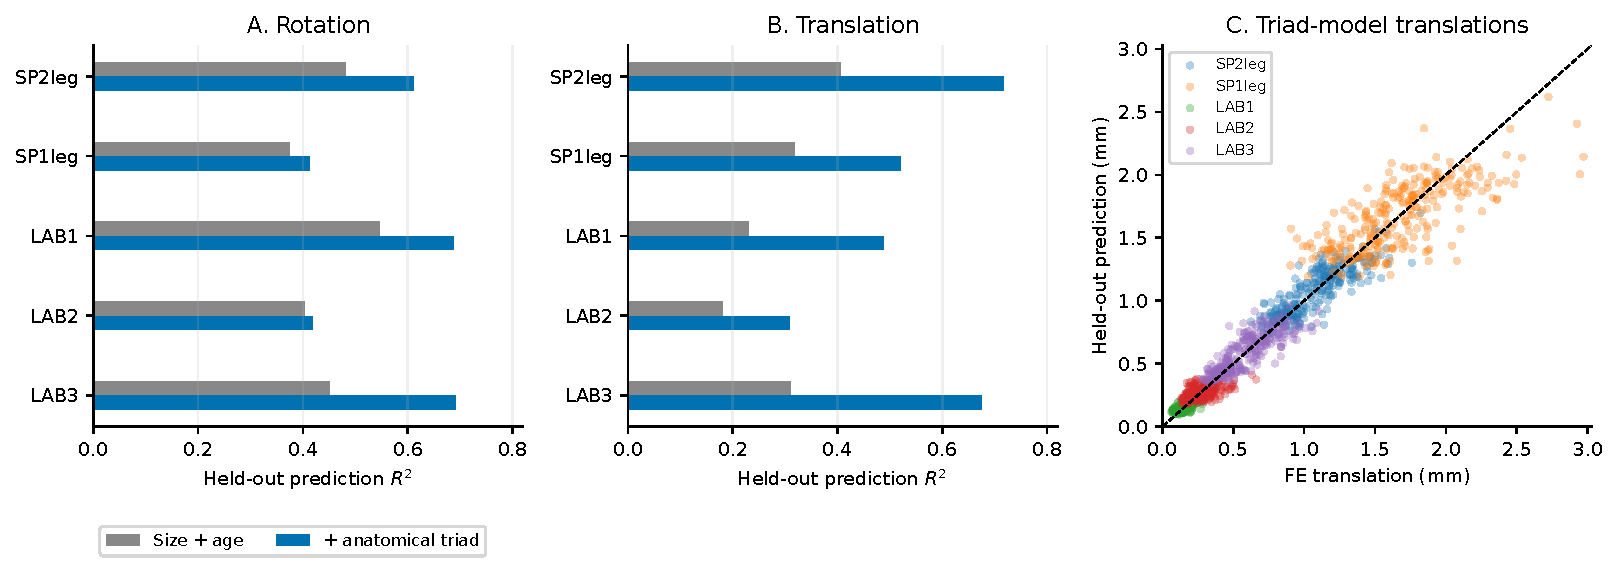
\includegraphics[width=\textwidth]{figures/Fig_prediction_subject_heldout.pdf}
\caption{\textbf{Predictive information in the anatomical triad.} (A,B) Held-out prediction $R^2$ for size and triad models, separately by load and endpoint. Each subject is held out from training in all loads. (C) Triad-model translations versus archived FE endpoints; each plotted prediction is averaged over validation repeats for display. The reported metrics in panels A,B and Table~\ref{tab:prediction} pool squared errors over repeats rather than using these averaged predictions. The dashed line is identity. Predictor selection was retrospective; these are internal validation results.}
\label{fig:prediction}
\end{figure}

\subsection{Unilateral support amplifies asymmetry at unchanged total force}
Redistributing a fixed total acetabular force changed the SIJ response. Under SP2leg and SP1leg, median rotation norms were 0.956$^\circ$ and 2.040$^\circ$, and median translations were 1.058 and 1.627~mm, respectively. Median bilateral translation asymmetry was 0.065~mm in SP2leg and 1.602~mm in SP1leg (Fig.~\ref{fig:loadprofiles}).
The paired SP1leg-minus-SP2leg median difference in rotation norm was $+1.048$ (95\% CI +1.004 to +1.102) degrees, $q<0.001$. The paired SP1leg-minus-SP2leg median difference in translation magnitude was $+0.582$ (95\% CI +0.559 to +0.603) mm, $q<0.001$. The paired SP1leg-minus-SP2leg median difference in translation asymmetry was $+1.509$ (95\% CI +1.445 to +1.568) mm, $q<0.001$. Redistributing the same 800~N total force therefore increased motion and, most prominently, bilateral asymmetry.

\begin{table}[htbp]
\centering
\caption{SIJ motion summaries across 278 subjects. Values are median [interquartile range]; component columns are absolute magnitudes.}
\label{tab:microsummary}
\StdTableInput{tables/generated/table3_micromotion_summary.tex}
\end{table}

\begin{figure}[htbp]
\centering
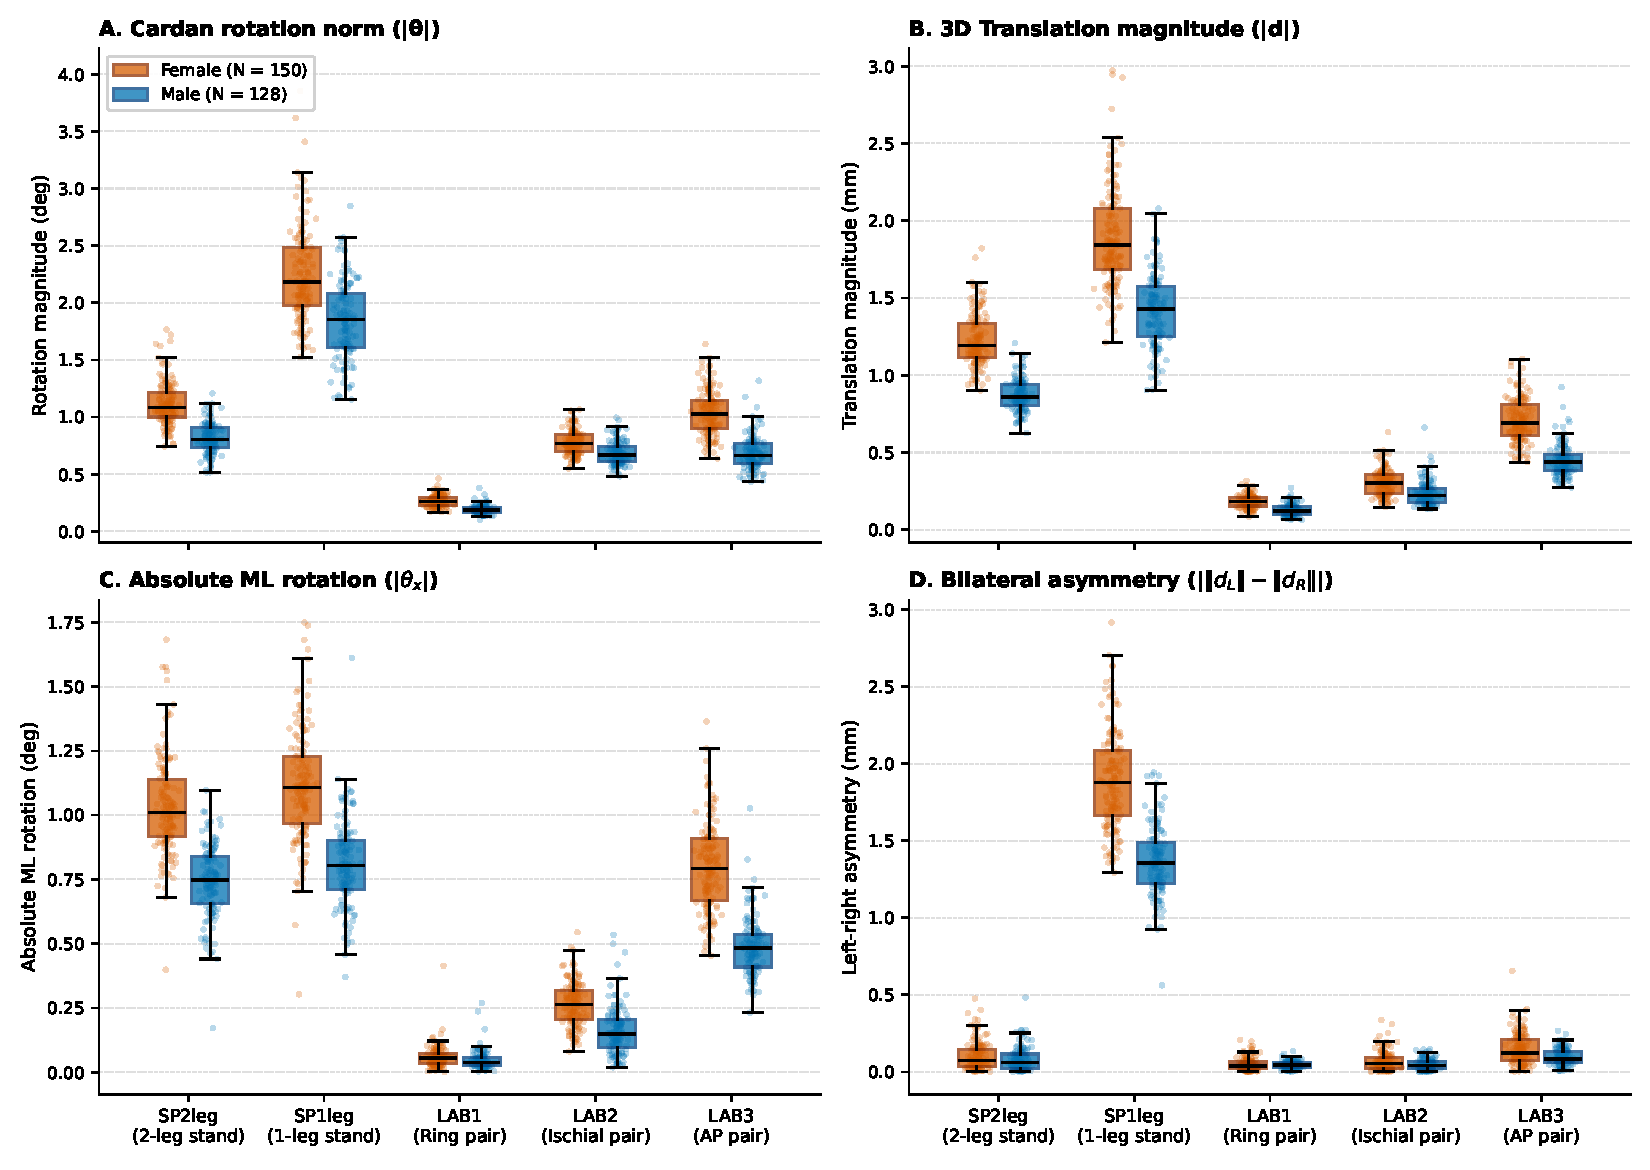
\includegraphics[width=\textwidth]{figures/Fig2_primary_load_profiles.pdf}
\caption{\textbf{Load-dependent motion and asymmetry.} Rotation-triplet norm, relative translation norm, absolute ML rotation and bilateral translation-magnitude asymmetry. Points are subjects; boxplots summarize each sex separately using medians and IQRs, with whiskers at 1.5 IQR. The numerical summaries in the text and Table~\ref{tab:microsummary} pool both sexes. Female and male groups use vermilion and blue. Jitter is deterministic. No signed nutation direction is inferred.}
\label{fig:loadprofiles}
\end{figure}
\subsection{Load application site selects distinct motion components}
The localized force pairs separated the response into distinct component patterns (Fig.~\ref{fig:directional}). Both transverse pairs reduced the absolute CC component relative to bilateral support, but the ML component increased only under LAB2: its paired median contrast was +0.052~mm (95\% CI +0.047 to +0.061, $q<0.001$), compared with $-0.007$~mm for LAB1 (95\% CI $-0.018$ to +0.002, $q=0.254$). Both also reduced the AP component. LAB3 increased the ML and AP components while reducing the CC component. The direct LAB2-minus-LAB1 contrasts confirmed larger ML and AP magnitudes (+0.058 and +0.111~mm), and a smaller CC magnitude ($-0.020$~mm), at the ischial application site; all three adjusted $q<0.001$ (Supplementary Table S12). Supplementary Table S1 gives all paired contrasts and adjusted probabilities. Component magnitudes quantify motion along the reporting axes; the arrows connect componentwise median contrasts and are not physical trajectories.

\begin{figure}[htbp]
\centering
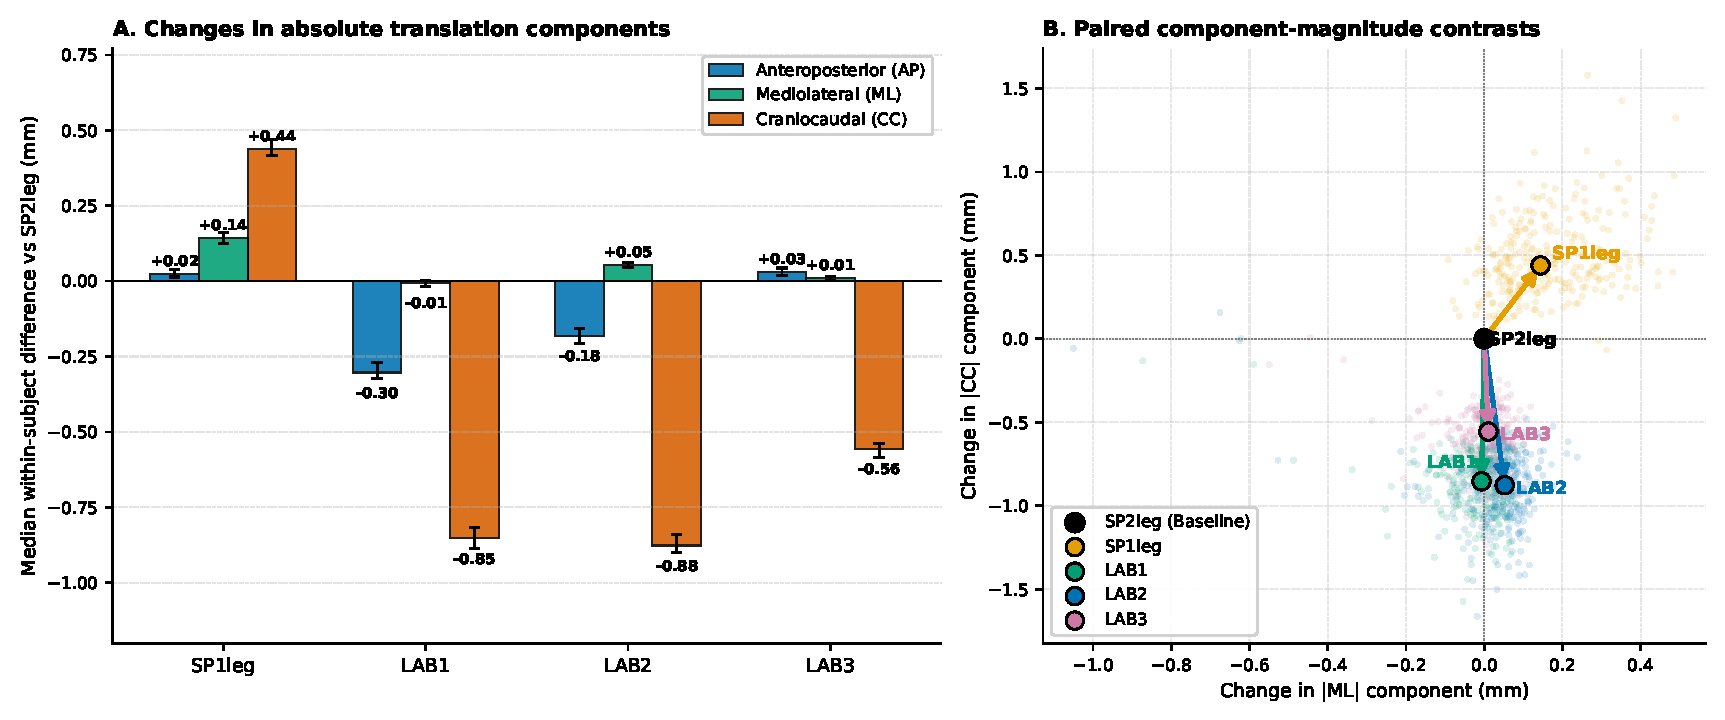
\includegraphics[width=\textwidth]{figures/Fig3_directional_rerouting.pdf}
\caption{\textbf{Paired absolute-component contrasts.} (A) Median within-subject differences from SP2leg, with bootstrap 95\% CIs. (B) Individual ML/CC contrast pairs and arrows to their componentwise medians. Positive values mean larger component magnitude, not outward joint motion. Corrected $q$ values are reported in Supplementary Table S1; intervals are pointwise, not simultaneous.}
\label{fig:directional}
\end{figure}
\FloatBarrier
\subsection{Direction limits the combination of scalar endpoint responses}
The controlled force redistribution isolated the information lost when endpoint motion is summarized only by magnitude (Fig.~\ref{fig:mixture}; Table~\ref{tab:mixture}). Both archived endpoint fields and their extracted kinematics were reproduced for all 278 subjects. Splitting each transverse force equally between the internal-ring and ischial patches ($w=0.5$) gave a median translation of 0.1587~mm. The median within-subject reduction relative to the scalar endpoint combination was 21.9\% (95\% bootstrap CI 20.0--23.7\%). At $w=0.25$, median translation was 0.1396~mm, below the endpoint medians of 0.1538 and 0.2549~mm, despite unchanged total force on each side.

At equal redistribution, scalar endpoint combination had RMSE 0.0580~mm against the motion re-extracted from mixed FE fields. Retaining signed endpoint vectors reduced this to 0.00021~mm. Across the three interior weights, scalar RMSE ranged from 0.0353 to 0.0580~mm, whereas vector RMSE ranged from 0.00014 to 0.00021~mm; the largest individual vector error was 0.00096~mm. The median of subjects' bilateral mean endpoint-vector cosines was 0.157, indicating substantial directional mismatch. These comparisons support directional cancellation as a mechanism limiting scalar load combination. They neither measure anatomy-only prediction on new subjects nor attribute the residual errors of the triad models to this mechanism.

\begin{table}[htbp]
\centering
\caption{Controlled transverse force redistribution. Translation is the cohort median after re-extraction from mixed fields. Directional reduction is the median within-subject percentage reduction relative to scalar endpoint combination; intervals are pointwise subject-bootstrap intervals. Scalar and vector estimates use individual FE endpoint information. RMSE is against the re-extracted mixed-field endpoint.}
\label{tab:mixture}
\StdTableInput{tables/prediction/table_mixture.tex}
\end{table}

\begin{figure}[htbp]
\centering
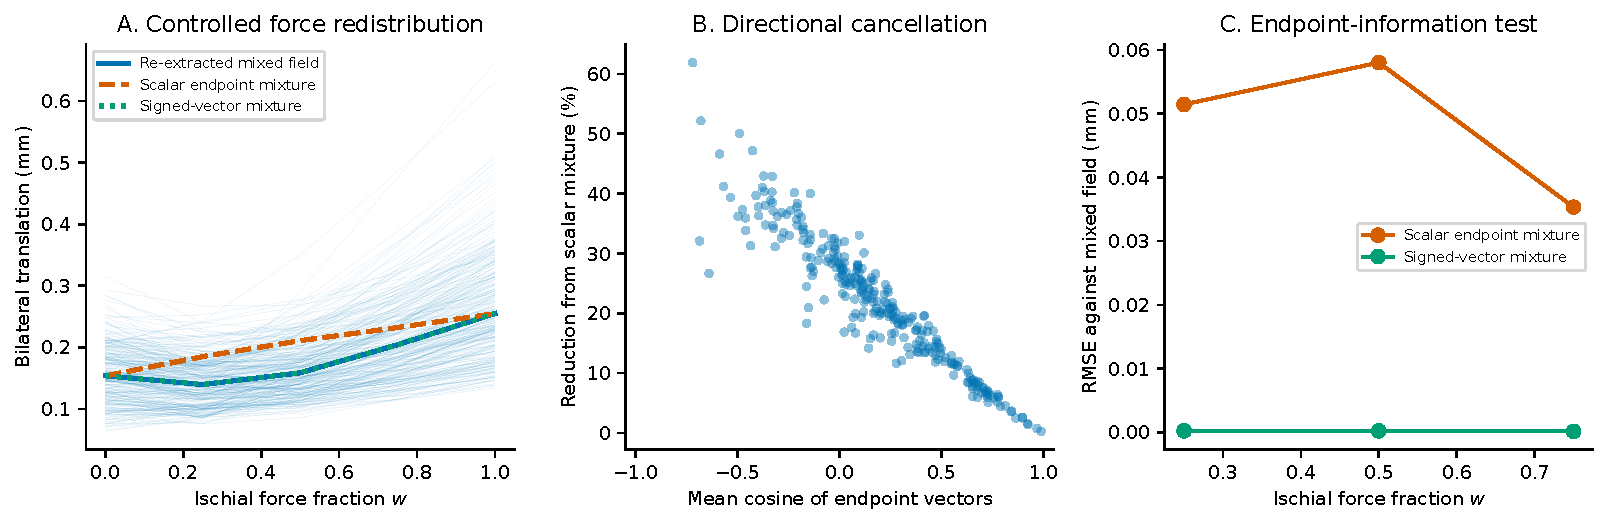
\includegraphics[width=\textwidth]{figures/Fig_load_mixture_mechanism.pdf}
\caption{\textbf{A directional limit to scalar response reduction.} Each 400~N transverse side force is progressively transferred from internal-ring to ischial patches, holding anatomy, tissues and total side force fixed. (A) Thin curves show subject translations re-extracted from exact mixtures of the FE displacement fields; thick curves show cohort medians for these translations and the two endpoint estimates. (B) Endpoint-vector alignment versus within-subject reduction at equal force redistribution. The cosine is averaged over the two sides; it is a directional diagnostic, not an independent predictor. (C) Scalar and signed-vector endpoint-combination errors. Field superposition is exact in the implemented linear system; combining extracted kinematic vectors is approximate, with its residual error measured.}
\label{fig:mixture}
\end{figure}
\FloatBarrier

\subsection{Selected morphometric adjustment attenuates sex-associated translation differences}
Adjustment for pelvic volume and the selected morphometric triad substantially attenuated the age-adjusted sex contrast under all three localized loads (Fig.~\ref{fig:sexeffects}). LAB1 female-minus-male translation coefficients were $+0.055$, $+0.040$ and $+0.013$~mm in M0, M1 and M2. The M2 interval was -0.005 to +0.031~mm ($p=0.166$, $q=0.566$). LAB2 female-minus-male translation coefficients were $+0.071$, $+0.041$ and $-0.031$~mm in M0, M1 and M2. The M2 interval was -0.078 to +0.016~mm ($p=0.192$, $q=0.566$). LAB3 female-minus-male translation coefficients were $+0.258$, $+0.212$ and $+0.002$~mm in M0, M1 and M2. The M2 interval was -0.060 to +0.064~mm ($p=0.950$, $q=0.950$). All three fully adjusted translation intervals spanned zero. The maximum non-intercept VIF in M2 was 5.55. Fully adjusted rotation intervals also spanned zero under all three loads (Supplementary Table S3).
The exploratory subpubic-angle comparison distinguished the pooled association from those within sex groups. For LAB1, the pooled Spearman correlation between subpubic angle and translation magnitude was $r_s=0.444$ ($p<0.001$). The male-only correlation was $r_s=-0.063$ ($p=0.480$). The female-only correlation was $r_s=-0.145$ ($p=0.077$). These exploratory correlations are uncorrected for multiplicity. Figure~\ref{fig:sexeffects} and Supplementary Table S3 report M2 estimates for both outcomes.

\begin{figure}[htbp]
\centering
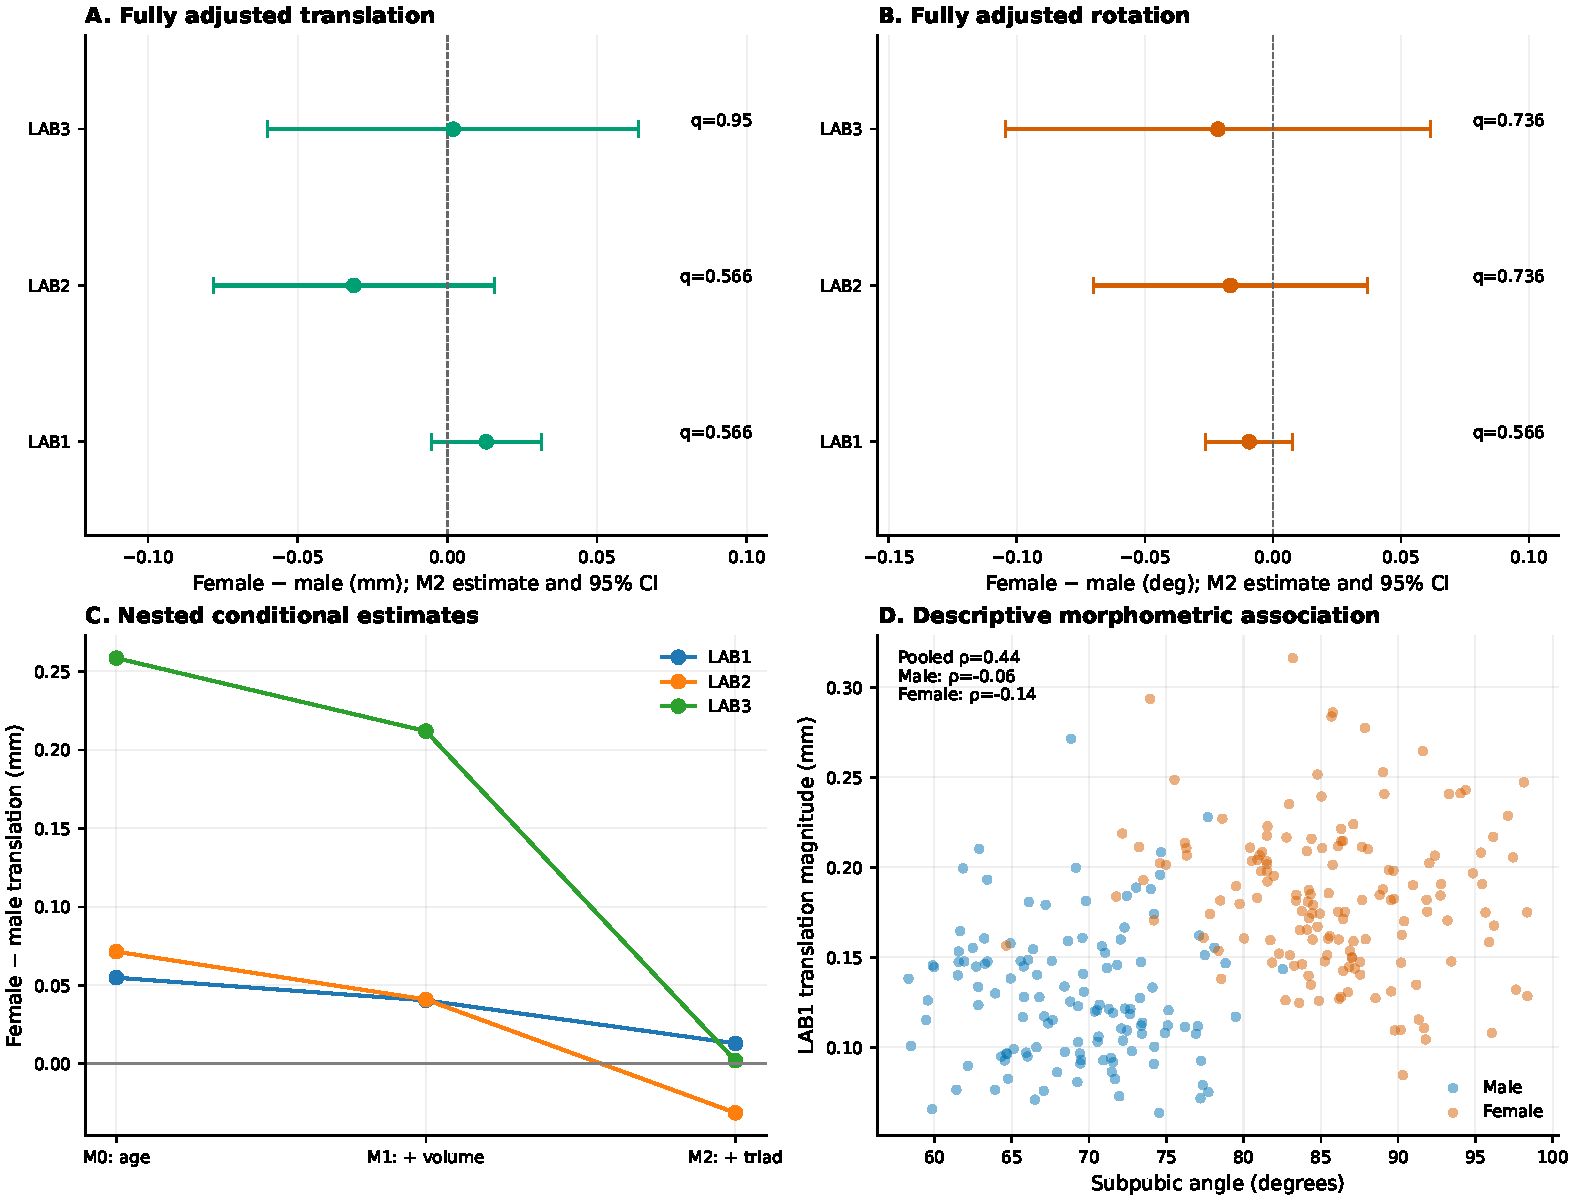
\includegraphics[width=\textwidth]{figures/Fig4_sex_effects_lab.pdf}
\caption{\textbf{Adjustment for volume and selected dimensions attenuates sex-associated translation differences.} (A,B) M2 female-minus-male coefficients with HC3 95\% CIs, shown on separate translation and rotation axes. Labels give BH-adjusted $q$ values across six tests. (C) Translation coefficients attenuate as pelvic volume and the selected triad enter the model; connecting lines compare specifications and are not causal pathways. (D) The positive pooled LAB1 subpubic-angle association is not reproduced within either sex. All M2 intervals span zero; this does not establish equivalence. M0 adjusts for age, M1 adds volume, and M2 adds the morphometric triad.}
\label{fig:sexeffects}
\end{figure}
\FloatBarrier
\subsection{Individual geometry preserves responses under standardized bone density}
Preserving individual geometry while standardizing the bone-density field retained individual motion closely. Across loads, translation had a minimum geometry-preserved/full identity-line $R^2$ of 0.9457 and maximum RMSE of 0.0280~mm. For rotation, the corresponding values were 0.8777 and 0.0318~degrees. Across five loads and five endpoints, geometry-preserved/full variance ratios ranged from 96.43\% to 120.61\% (median 100.68\%), compared with 0.014\% to 5.789\% (median 0.244\%) for density-preserved/full ratios. These are model-variant comparisons, not an additive variance decomposition (Fig.~\ref{fig:variance}; Supplementary Table S2). Small cohort-average errors do not bound individual errors: under SP2leg, translation absolute error had a 95th percentile of 0.0486~mm and a maximum of 0.2195~mm (Supplementary Table S11).

\begin{figure}[htbp]
\centering
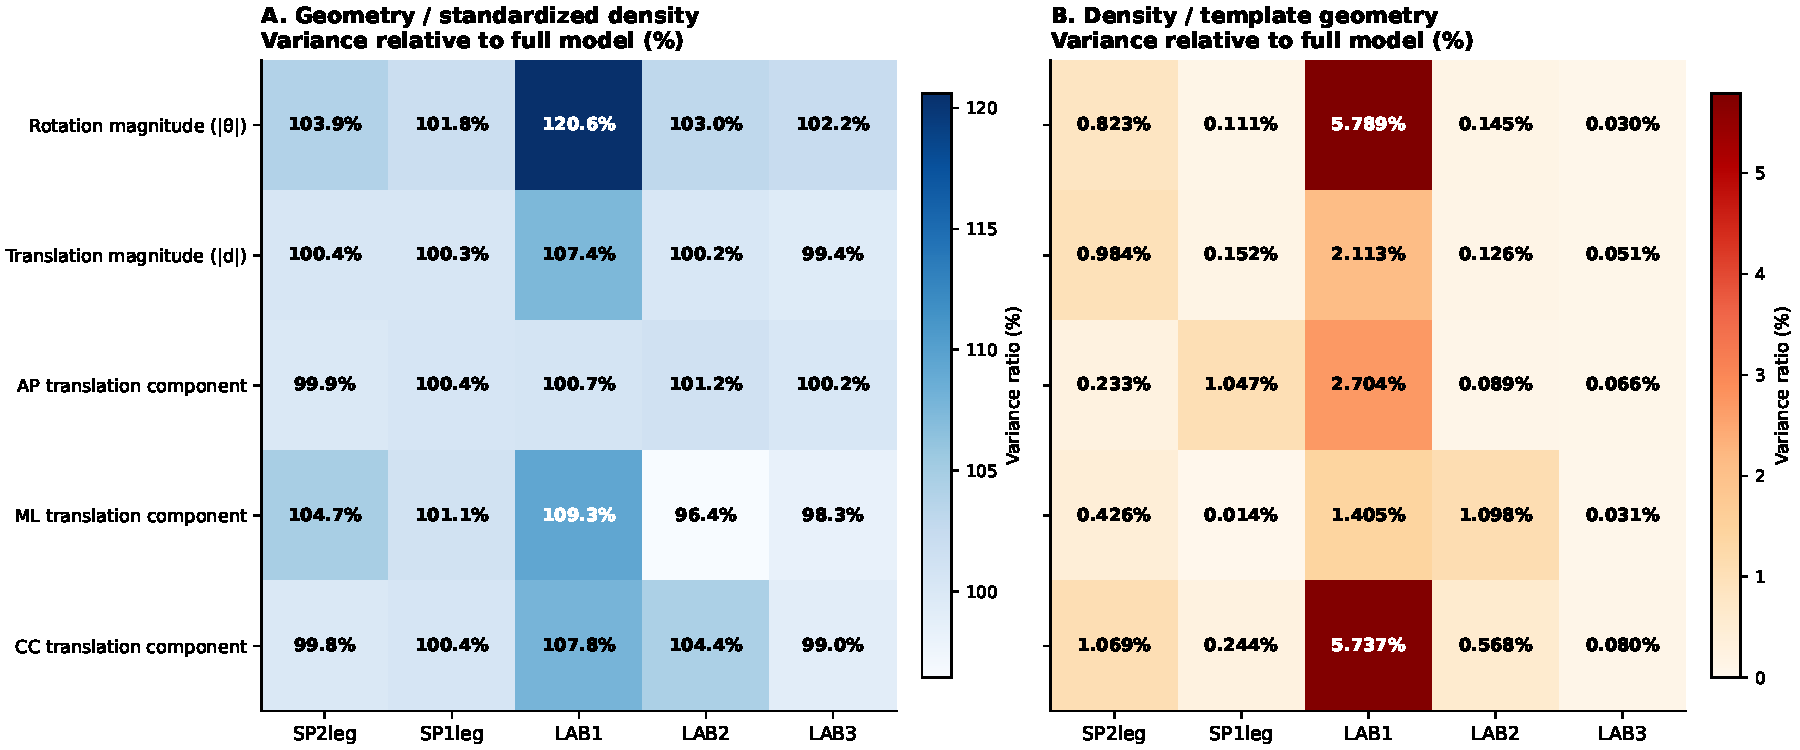
\includegraphics[width=\textwidth]{figures/Fig5_variance_channels.pdf}
\caption{\textbf{Retaining individual geometry preserves between-subject variation.} (A) Geometry-preserved / standardized-density and (B) density-preserved / template-geometry sample variances, each divided by the full-model variance, in percent. Five endpoints are shown. Color scales differ between panels and follow their actual data ranges. Values above 100\% are allowed. Subject-level agreement complements these variance summaries (translation RMSE $\leq0.0280$~mm; minimum identity-line $R^2=0.9457$). Bootstrap intervals and agreement diagnostics are provided in Supplementary Table S2; neither panel represents variance explained by an independent causal factor.}
\label{fig:variance}
\end{figure}
\subsection{Exploratory size associations depend on anatomical adjustment}
All 20 sex-specific conditional log-volume slopes were negative after adjustment for age and the triad (range $-1.062$ to $-0.366$, maximum slope $q=0.002$). Sex--volume interaction $q$ values ranged from 0.343 to 0.699. In matched models omitting the triad, all slope estimates remained negative, but the maximum adjusted slope $q$ increased to 0.291; for example, the LAB1 female translation slope changed from $-1.003$ to $-0.481$. These are conditional associations, not estimates from uniformly scaled geometries. The full coefficients, adjustment comparison and exploratory dimensional references are provided in Supporting Information (Tables S9 and S13; Figures S1 and S3). Pooled coefficients using subject-clustered covariance are in Table S5.

\subsection{Sensitivity of motion extraction}
In six subjects selected at approximately evenly spaced cohort row indices (30 subject--load comparisons), replacing affine sacral correction with rigid-only correction changed bilateral rotation norms by at most 0.0229$^\circ$ and translation magnitudes by at most 0.0055~mm. This subset diagnostic does not bound errors in the remaining cohort (Supplementary Table S6).

\FloatBarrier
\section{Discussion}
Pelvic mechanical response was structured by anatomical scale and individual architecture, and its expression depended strongly on load path. Size showed a consistent inverse conditional relationship with motion across loads. Adjustment for pelvic volume and the selected morphometric triad substantially attenuated sex-associated translation differences under localized loading, while preserving individual geometry under standardized bone density retained subject-specific responses closely. Redistributing force or changing its application site nevertheless altered the magnitude and component pattern of motion. These observations support an anatomically resolved description of response under specified loading.

\subsection*{Conditional mechanical scaling}
The 20 negative sex-specific volume slopes, all retained after multiplicity correction, make size a common mechanical context for the anatomical comparisons. SP2leg slopes lay numerically near the simple dimensional references of $-1/3$ for translation and $-2/3$ for rotation. Several localized-load estimates were numerically steeper, including LAB1 rotation and LAB2 translation; this is a descriptive comparison across loads.

The reference values follow elementary dimensional reasoning: for geometrically similar linear-elastic structures at fixed force $F$ and modulus $E$, translation scales as $u\sim F/(EL)\propto V^{-1/3}$, and rotation as $\theta\sim u/L\propto V^{-2/3}$. These are heuristic dimensional references. The fitted slopes describe changes in volume at fixed values of the selected morphometric dimensions; the dimensional references describe uniform geometric scaling. Why some localized-load estimates are numerically steeper remains unresolved. The pelvis is a jointed structure with heterogeneous tissues and varying proportions. Fixed ligament spring parameters and cartilage properties do not impose geometric similarity across sizes. Geometry-dependent force moments, heterogeneous density fields and conditional adjustment for other dimensions could also contribute to the load-specific slopes. Their contributions remain to be tested.

The slopes describe conditional mechanical scaling under standardized forces. Physiological scaling with body-mass-dependent loading was not evaluated.

\subsection*{Size, shape and sex-associated response}
The female and male groups differed in several dimensions: female pelves had lower total bone volume but greater mean inlet depth, interspinous width and subpubic angle (Table~\ref{tab:cohort}). Sex groups therefore differ in both size and proportions. Anatomical evidence distinguishes allometric differences in overall proportions from largely non-allometric differences in subpubic angle \citep{Fischer2017}; local auricular shape also differs between sexes \citep{Nishi2020}. Earlier representative-model comparisons of standing SIJ mechanics \citep{Joukar2018} establish relevant prior evidence, while the present cohort examines how population contrasts change with explicit anatomical adjustment and loading context. Adding pelvic volume and the selected morphometric triad reduced the female translation coefficients from +0.055 to +0.258~mm across localized loads to -0.031 to +0.013~mm. All three fully adjusted translation intervals under localized loading included zero. Coefficient attenuation quantifies the change in the sex-associated contrast after anatomical adjustment. Sex equivalence and causal mediation were not tested.

The subpubic-angle association depended on whether subjects were pooled or stratified by sex. The positive pooled correlation with LAB1 translation was not reproduced within either sex: both within-sex estimates were weakly negative and their tests did not reject zero correlation. The selected triad represents a subset of pelvic architecture. Out-of-sample predictive performance was not evaluated. External assessment should examine anatomical overlap between sexes, collinearity and performance beyond this cohort.

\subsection*{Geometry retains the subject-specific mechanical response}
The matched geometry--density comparison quantified the preservation of individual responses after density standardization. Retaining individual geometry with the spatially varying median density field gave translation RMSE no greater than 0.028~mm and a minimum identity-line $R^2$ of 0.946. The minimum identity-line $R^2$ for rotation was 0.878. The near-100\% geometry-preserved/full variance ratios and small density-preserved/full ratios were consistent with these paired comparisons. CT-osteoabsorptiometry showed limited differences in mineralization patterns across auricular shape categories, although larger surfaces had higher iliac mineralization \citep{Poilliot2023}. Those observations provide context on long-term subchondral adaptation. Individual geometry may be prioritized when modeling these joint-motion endpoints. The acceptable degree of density simplification depends on the error tolerance.

This hierarchy is conditional on the passive static model and its implemented density--modulus law, including a low-density modulus floor. Cartilage properties, ligament properties and pretension were fixed. Ligament pretension can substantially affect SIJ predictions \citep{Heyland2025}, and introducing individual soft-tissue variation could change the relative contributions. Under these constitutive assumptions, standardizing the represented bone-density field produced substantially smaller changes in these SIJ-motion endpoints than standardizing subject geometry. The constant low-density modulus branch suppresses represented stiffness variation and may contribute to this contrast; the comparison does not quantify the effect of density under alternative constitutive laws.

\subsection*{Load path determines how architecture is expressed}
SIJ mobility depended on force distribution. Redistributing 800~N from bilateral to unilateral acetabular support increased translation and rotation and strongly amplified bilateral asymmetry. The total applied force was unchanged, but its moments and route through the ring changed. This gives a population-level mechanical context to established accounts of SIJ load transfer \citep{Snijders1993,Vleeming2012}.

Application site was also consequential. Both transverse force pairs reduced the craniocaudal component relative to bilateral support. The mediolateral contrast with bilateral support was positive for the ischial pair, whereas the interval for the internal-ring pair included zero. These comparisons partly supported the shared transverse-redistribution hypothesis and described distinct component patterns; a direct contrast between the two application sites was not reported.

\subsection*{Implications for functional anatomy}
Overall size was inversely associated with motion magnitude, preserving individual geometry retained subject-specific responses, and load path altered the expressed motion pattern. Sex captures part of the population variation in anatomical dimensions. The present analyses connect whole-pelvis size and dimensions to load-dependent motion and test a geometry-preserving density simplification. The evidence supports describing pelvic function through scale, architecture and loading context together.

Covariation of stature and pelvic shape provides anatomical context for obstetric dimensions \citep{Fischer2015}. The present endpoints quantify relative SIJ motion. Signed joint opening and birth-canal expansion were not measured. Their evaluation under delivery conditions requires direct surface-separation and canal measurements, together with fetal contact and soft-tissue interactions \citep{ChenGrimm2021}.

\subsection*{Limitations and experimental tests}
The model represents passive, static mechanics with a constrained sacrum, nominal cartilage properties and linearized ligaments, without muscle activation or frictional contact. The density comparison inherits these choices. Absolute motion magnitudes depend on using the zero-displacement anatomical configuration rather than an equilibrated pretension-only reference; all paired load comparisons use the same reference convention and prescribed pretension. The cohort spans ages 16--91 and does not specifically represent pregnant or laboring women; pregnancy-related adaptation, parity, pain and delivery outcomes were not analyzed. The retrospective selection of dimensions and comparisons also limits confirmatory interpretation.

Affine sacral correction removes sacral strain as well as rigid drift. The rigid-only sensitivity check showed small endpoint changes in the six subjects examined; its coverage was limited to this subset. Sampling intervals exclude constitutive, anatomical-interpolation and boundary-condition uncertainty. A previous subject-specific pelvic model was validated against cortical strains \citep{Anderson2005}. Physiological SIJ kinematics remain unvalidated in the present cohort. Further assessment of mesh and anatomical-interpolation accuracy, together with independent measurements under matched loads, would strengthen numerical and experimental validation, particularly given the difficulty of measuring small SIJ motions \citep{Goode2008}.

The resulting experimental predictions are specific: unilateral loading should increase bilateral asymmetry at matched total acetabular force, and transverse forces at the internal ring and ischial tuberosities should produce different component responses. Tests should measure signed SIJ surface separation alongside the reported point-motion endpoints. Comparing subject-specific and standardized density assignments against those measurements would test the proposed simplification, while introducing measured cartilage, ligament and pretension variation would test its scope. Independent specimens and loading configurations are needed to determine how far the anatomical relationships generalize.

\section{Conclusion}
Pelvic volume, age and three anatomical measures predicted a useful but load-dependent part of population SIJ motion in internal subject-held-out validation. The triad improved translation prediction beyond size in all five loads, while its contribution to rotation varied. A controlled within-subject experiment identified a separate limit: scalar endpoint magnitudes lost directional information needed to combine responses when the same forces were redistributed between application sites. Retaining signed vectors nearly recovered the mixed-load response. These findings support compact anatomical prediction under specified loads and motivate directional response models for load transfer. Generalization requires independent anatomy and experimental kinematic validation, including variation in soft-tissue properties.


\appendix
\section{Mathematical formulation and verification}
\label{app:mathematical_formulation}

\subsection{Implementation and correspondence checks}
\label{app:implementation_checks}
Subject landmarks were obtained by thin-plate-spline RBF interpolation of template-to-subject displacements (10 neighbors; smoothing parameter 100). These morphometric interpolation settings differ from those used for the FE surface reconstruction. Repeated calculation of the eight measures for all 278 subjects agreed within $10^{-8}$~mm or degrees.

Reference-to-reference checks were below $10^{-8}$ in degrees and mm for every subject. Node ordering was checked against the reference displacement fields for all five load cases. Geometry and displacement were evaluated with the same RBF parameters used for surface reconstruction. Subject pairing across the three variants follows the common row indices of the geometry and density inputs. This pairing was checked for consistency of row ordering; an independent identifier-based check was not available.

The FE displacement and geometry spaces were continuous vector P1 on linear tetrahedra, with DG0 material fields and integration degree 6. The linear system used PETSc \texttt{KSPPREONLY}, \texttt{PCLU} and MUMPS, with option prefix \texttt{elas\_}. Configured relative and absolute tolerances were $10^{-10}$ and $10^{-12}$, with an iteration limit of 1000; the selected direct factorization does not use an iterative residual stopping test. The implementation records PETSc's convergence reason. RBF transfer of the geometry displacement to FE nodes used 10 neighbors and smoothing 50; transfer from FE nodes to the measurement geometry used 10 neighbors and zero smoothing.

\subsection{Reference mapping and equilibrium}
Let $\Omega_0$ be the FE template and $\boldsymbol\chi_i(\mathbf X)=\mathbf X+\boldsymbol\phi_i(\mathbf X)$ the unloaded subject geometry. The anatomical registration is bijective; RBF interpolation represents its established displacement map on the FE template. The anatomical mapping and the elastic displacement are different fields. With $\mathbf F_i=\mathbf I+\nabla_X\boldsymbol\phi_i$ and $J_i=\det\mathbf F_i$, the physical small-strain tensor is
\begin{equation}
\boldsymbol\varepsilon_i(\mathbf u)=\operatorname{sym}(\nabla_X\mathbf u\,\mathbf F_i^{-1}).
\end{equation}
Here $\nabla_X\mathbf u$ differentiates the displacement represented on the template; $\operatorname{sym}\mathbf B=(\mathbf B+\mathbf B^T)/2$. Volume integration satisfies $dV_i=J_i\,dV_0$. Thus, for example, the elastic term on the template is $\int_{\Omega_0}(\mathbf C_i\boldsymbol\varepsilon_i(\mathbf u)): \boldsymbol\varepsilon_i(\mathbf v)\,J_i\,dV_0$. For physical coordinates in mm, find the discrete displacement $\mathbf u_h$ such that, for every test displacement $\mathbf v_h$, the weak problem is
\begin{equation}
\int_{\Omega_i}\mathbf C_i\boldsymbol\varepsilon(\mathbf u):\boldsymbol\varepsilon(\mathbf v)\,dV
+\int_{\Gamma_{S1,i}}\gamma\,\mathbf u\cdot\mathbf v\,dS
+\mathbf v_h^T\mathbf K_{lig,i}\mathbf u_h
=\int_{\Gamma_{load,i}}\mathbf t\cdot\mathbf v\,dS+\mathbf v_h^T\mathbf f_{pre,i}.
\end{equation}
Here $\mathbf C_i$ is the isotropic elasticity tensor, $\mathbf t$ is the prescribed surface traction, and $\mathbf u_h,\mathbf v_h$ are nodal coefficient vectors in the spring terms. In each tissue, $\boldsymbol\sigma=2\mu\boldsymbol\varepsilon+\lambda\operatorname{tr}(\boldsymbol\varepsilon)\mathbf I$, with $\mu=E/[2(1+\nu)]$ and $\lambda=E\nu/[(1+\nu)(1-2\nu)]$. The surface penalty has units N/mm$^3$, because its associated traction is $\gamma\mathbf u$ in N/mm$^2$. It imposes an approximate fixed boundary, not exact $\mathbf u=0$. The ligament stiffness and pretension terms are required for consistency with the assembled solver. For one spring segment of length $L$, direction $\mathbf e$, assigned stiffness $k$ and pretension $T$, its directional stiffness is
\begin{equation}
\mathbf W=k\mathbf e\mathbf e^T+(T/L)(\mathbf I-\mathbf e\mathbf e^T).
\end{equation}
This matrix is assembled with opposite off-diagonal blocks at its two endpoints. It is a linearized spring representation without tension-only switching.

The surface measure obeys $dS_i=J_{surf,i}dS_0$, where
\begin{equation}
J_{surf,i}=J_i\|\mathbf F_i^{-T}\mathbf n_0\|,\qquad
\mathbf t=\frac{\mathbf F^{tot}}{\int_{\Gamma_{load,0}}J_{surf,i}\,dS_0}.
\end{equation}
Thus the applied physical force integral equals $\mathbf F^{tot}$. The penalty and load integrals use the corresponding mapped surface measures. The force vectors are listed in Table~\ref{tab:loads}; their global axes are not assumed identical to the PCA reporting axes below.

\subsection{Unloaded and loaded surfaces}
Let $\mathbf X_j$ be surface template nodes. The two point clouds used for kinematics are
\begin{equation}
\mathbf p^0_{ij}=\mathbf X_j+\boldsymbol\phi_i(\mathbf X_j),\qquad
\mathbf p^1_{i\ell j}=\mathbf p^0_{ij}+\mathbf u_{i\ell}(\mathbf X_j).
\end{equation}
Both use identical topology and point correspondence. Here ``unloaded'' denotes the geometric reference with zero elastic displacement, not a separately equilibrated pretension-only state. The loaded field includes both the prescribed external load and the ligament pretension right-hand side. Comparing $\mathbf X_j$ with $\mathbf p^1_{i\ell j}$ would incorrectly include subject morphology in the measured motion. Geometry was reconstructed with two-stage interpolation: template-to-FE mapping (10 neighbors, smoothing 50) followed by FE-to-surface mapping (10 neighbors, zero smoothing). Elastic displacement fields use the latter interpolation. Cached sparse interpolation weights implement the same linear RBF evaluation; numerical comparisons against direct RBF evaluation check this equivalence.

\subsection{Pelvis-aligned reporting frame}
The origin $\mathbf o$ is the centroid of the unloaded surface. The initial ML axis is the dominant eigenvector of the point-cloud covariance, with deterministic sign. The symmetry-plane routine uses this PCA approximation; it does not optimize reflection symmetry. Project the centered points onto its orthogonal plane and take the leading in-plane singular vector. Orthogonalization gives $\hat{\mathbf z}$, followed by
\begin{equation}
\hat{\mathbf y}=\frac{\hat{\mathbf z}\times\hat{\mathbf x}}{\|\hat{\mathbf z}\times\hat{\mathbf x}\|},\qquad
\hat{\mathbf z}=\hat{\mathbf x}\times\hat{\mathbf y},\qquad
\mathbf P=[\hat{\mathbf x},\hat{\mathbf y},\hat{\mathbf z}].
\end{equation}
The ML and AP axes are simultaneously reversed if needed so that ML points from the left to right ilium centroids. This construction is orthonormal and right-handed but does not independently anchor the AP/CC signs to anatomical landmarks. Absolute components are therefore used for comparisons. No clinical nutation sign is inferred from the stored $\alpha_x$ sign.

\subsection{Affine correction, regions and rigid fits}
Fit the sacral point correspondence by ordinary least squares,
\begin{equation}
(\mathbf A_S,\mathbf b_S)=\arg\min_{\mathbf A,\mathbf b}\sum_{j\in S}
\|\mathbf p^1_j-\mathbf A\mathbf p^0_j-\mathbf b\|^2,
\qquad \mathbf q_j=\mathbf A_S^+(\mathbf p^1_j-\mathbf b_S),
\end{equation}
where $+$ denotes the Moore--Penrose pseudoinverse. This removes fitted affine sacral deformation, including stretch and shear; it is not only a change of rigid observer frame.

For each side, first restrict both point clouds to that side of the reporting-frame midplane (falling back to the entire bone if this set is empty). Select sacral and iliac points within 5~mm of the opposing restricted point cloud. If fewer than 80 points qualify, use up to the nearest 80 available points. Distances are between discrete points rather than continuous articular surfaces. For each bone ROI, the rigid fit maps $\mathbf p^0$ to $\mathbf q$. With centered row matrices $\widetilde{\mathbf P}_B,\widetilde{\mathbf Q}_B$,
\begin{equation}
\widetilde{\mathbf P}_B^T\widetilde{\mathbf Q}_B=\mathbf U\boldsymbol\Sigma\mathbf V^T,
\quad \mathbf R_B=\mathbf V\operatorname{diag}(1,1,\det(\mathbf V\mathbf U^T))\mathbf U^T,
\quad \mathbf t_B=\bar{\mathbf q}_B-\mathbf R_B\bar{\mathbf p}^0_B.
\end{equation}
The fit is repeated after excluding the largest 10\% residuals, using two trimming iterations. Trimming reduces outlier influence but does not validate the ROI as a physical contact patch.

\subsection{Relative rotation and translation}
For sacral and iliac fits $S,I$,
\begin{equation}
\mathbf R_{rel}=\mathbf R_S^T\mathbf R_I,\qquad
\mathbf R_{loc}=\mathbf P^T\mathbf R_{rel}\mathbf P
=\mathbf R_z(\gamma_z)\mathbf R_y(\beta_y)\mathbf R_x(\alpha_x).
\end{equation}
The fixed-axis $xyz$ extraction, for zero-based matrix indices away from gimbal lock, is
\begin{equation}
\alpha_x=\operatorname{atan2}(R_{21},R_{22}),\quad
\beta_y=\arcsin[-\operatorname{clip}(R_{20},-1,1)],\quad
\gamma_z=\operatorname{atan2}(R_{10},R_{00}).
\end{equation}
At $\beta_y=\pm\pi/2$, choose $\gamma_z=0$ and
$\alpha_x=\operatorname{atan2}[-\operatorname{sign}(R_{20})R_{01},R_{11}]$.
In implementation, the equivalent stable expression $\beta_y=\operatorname{atan2}(-R_{20},\sqrt{R_{00}^2+R_{10}^2})$ is used, with the singular branch restricted to vanishing cosine. The singular branch is included for completeness; physiological small-angle outputs should remain far from it. Matrix reconstruction tests cover both branches.

For the unloaded sacral ROI centroid $\mathbf p_c$, the reported displacement is
\begin{equation}
\mathbf d=\mathbf P^T[(\mathbf R_I-\mathbf R_S)\mathbf p_c+\mathbf t_I-\mathbf t_S].
\end{equation}
It evaluates the difference of two fitted maps at a common reference point, expressed in the unloaded pelvic axes after affine correction. It is not the translational parameter of $T_S^{-1}T_I$. In fact, with $\mathbf t_{rel}=\mathbf R_S^T(\mathbf t_I-\mathbf t_S)$,
\begin{equation}
\mathbf d=\mathbf P^T\mathbf R_S\big[(\mathbf R_{rel}-\mathbf I)\mathbf p_c+\mathbf t_{rel}\big].
\end{equation}
This identity makes explicit the distinction between the relative rigid transform and the reported point-displacement difference. It is neither the distance between opposing articular surfaces nor a displacement along a surface normal. The bilateral summaries are
\begin{align}
|\boldsymbol\theta|&=\tfrac12\sum_{s=L,R}(\alpha_{x,s}^2+\beta_{y,s}^2+\gamma_{z,s}^2)^{1/2}, &
|\mathbf d|&=\tfrac12\sum_{s=L,R}\|\mathbf d_s\|,\\
|d_k|&=\tfrac12(|d_{k,L}|+|d_{k,R}|), &
A_d&=\big|\|\mathbf d_L\|-\|\mathbf d_R\|\big|.
\end{align}
Angles are converted to degrees before reporting. The exact principal rotation angle would instead be $\arccos[(\operatorname{tr}\mathbf R_{rel}-1)/2]$ with numerical clipping. The Cardan norm approximates it at small angles and depends on the chosen axes and sequence.

\subsection{Conditional size scaling}
Pelvic bone volume was calculated by summing the volumes of the selected left and right hip-bone bodies and sacrum, using mapped surface geometry and converting mm$^3$ to cm$^3$. These are whole-bone geometric volumes, not birth-canal volume or a direct integral of cortical tissue. The size factor is $s_i=(V_i/V_{template})^{1/3}$. Therefore a log-volume slope $b$ becomes $3b$ under log scale, with identical fitted responses and tests.

For the sex-interaction log model, $b_M=\beta_v$ and $b_F=\beta_v+\beta_{v:s}$. The female slope variance is
\begin{equation}
\operatorname{Var}(b_F)=\operatorname{Var}(\beta_v)+\operatorname{Var}(\beta_{v:s})+2\operatorname{Cov}(\beta_v,\beta_{v:s}).
\end{equation}
Reported intervals use this full covariance. Exponentiating a fitted log response gives a conditional geometric mean, not an unbiased arithmetic mean. Figure~\ref{fig:allometry} reports slopes from this model. Supplementary Figure S1 shows its conditional geometric-mean curves with age and the morphometric covariates set to their cohort means.

\subsection{Statistical estimands and uncertainty}
All logarithms are natural logarithms of numerical values in the stated units: $\log V$ abbreviates $\log[V/(1\,\mathrm{cm}^3)]$, and $\log Y$ uses 1~mm or 1 degree as the reference unit. Changing these reference units changes intercepts, but not the sex-specific volume slopes. Standardized predictors are $z_i=(x_i-\bar x)/s_x$, where $s_x$ is the cohort sample standard deviation; for log volume, the logarithm is taken before standardization.

For design matrix $\mathbf Z$, OLS residuals $e_i$ and leverage $h_{ii}$, the HC3 covariance estimator is
\begin{equation}
\widehat{\operatorname{Cov}}_{HC3}(\widehat{\boldsymbol\beta})=
(\mathbf Z^T\mathbf Z)^{-1}\mathbf Z^T
\operatorname{diag}\!\left[\frac{e_i^2}{(1-h_{ii})^2}\right]
\mathbf Z(\mathbf Z^T\mathbf Z)^{-1}.
\end{equation}
For any coefficient contrast $\mathbf c$, its estimate is $\mathbf c^T\widehat{\boldsymbol\beta}$ and standard error is $[\mathbf c^T\widehat{\operatorname{Cov}}_{HC3}\mathbf c]^{1/2}$. Reported Wald intervals use the normal critical value (approximately 1.96). The volume slopes are conditional elasticities: holding the other predictors fixed, multiplying volume by $a>0$ multiplies the fitted geometric-mean response by $a^b$.

For a paired contrast $\Delta_i$, the reported effect is $\operatorname{median}_i\Delta_i$, not the difference between two marginal medians. With $n_*$ nonzero differences and $B=\sum_i\mathbb 1(\Delta_i>0)$, the two-sided exact sign test uses $B\sim\operatorname{Binomial}(n_*,1/2)$ under the null of balanced signs. For a continuous difference distribution this is a test of zero median; excluding exact zeros conditions on nonzero differences. Bootstrap intervals are percentile intervals obtained by resampling subjects, preserving the paired observations. They are pointwise intervals, whereas the reported $q$ values apply Benjamini--Hochberg adjustment within the specified test families; these two summaries need not cross their respective thresholds together.


\section*{Funding}
This work was supported by the Czech Science Foundation (GA\v{C}R; Grant No.\ 24-10862S). The funder had no role in study design, data analysis or interpretation, manuscript preparation, or the decision to submit the article for publication.

\section*{Author contributions}
CRediT authorship contribution statement. Petr Heny\v{s}: Conceptualization; Methodology; Software; Formal analysis; Investigation; Data curation; Visualization; Funding acquisition; Writing -- original draft; Writing -- review \& editing. Niels Hammer: Supervision; Writing -- review \& editing.

\section*{Declaration of competing interest}
The authors declare no competing interests.

\section*{Supporting information}
Supporting Information provides paired prediction gains and benchmark errors, statistical definitions, direct application-site contrasts, density-standardization error tails, variance ratios, sex models, exploratory conditional volume associations and extraction sensitivity diagnostics.

\section*{Data Availability Statement}
The source anonymized CT images, segmentations and standardized anatomical geometries are available through BoneDat \citep{HenyssKuchar2025BoneDat}, with source data indexed by the \href{https://doi.org/10.5281/zenodo.15189761}{BoneDat dataset record}. The present study's derived morphometric tables, subject-level motion endpoints, held-out predictions, load-mixture results, machine-readable model estimates and analysis code have not been deposited in a public repository. The Supporting Information provides the statistical definitions, component contrasts, variance ratios, model estimates and sensitivity analyses reported here. The BoneDat record identifies the source imaging and anatomical data, not a repository for this study's FE results or code.

\section*{Declaration of generative AI and AI-assisted technologies in the manuscript preparation process}
OpenAI Codex (GPT-6, OpenAI) assisted with literature searches, manuscript organization and drafting, and development of analysis and visualization code. Its contribution to the research workflow is described in the Methods. Both authors reviewed and approved the resulting text and outputs and accept responsibility for the article's accuracy, interpretation and integrity.

\bibliographystyle{bib/apalike-doi}
\bibliography{bib/refs}

\end{document}
